\documentclass[12pt]{scrreprt}

%\documentclass[a4paper, 12pt, oneside]{scrbook}

%Eingaben

\usepackage[latin1, utf8]{inputenc}

\usepackage[T1]{fontenc}

\usepackage[ngermanb, english]{babel}

\usepackage{amsmath}
\usepackage{amsthm}
\usepackage{ulem}
%Layout

\usepackage{lmodern}

\usepackage{hyperref}

\usepackage[all]{hypcap} %Bei Verlinkungen auf Bilder die obere Grenze des Bildes verkinken.

%Für die Erzeugung von Graphiken

\usepackage{tikz}

%\usepackage{graphicx}

%Quellcode

\usepackage{listings}
\usepackage{graphicx}
\usepackage{color}

\lstdefinestyle{Shell}{delim=[il][\bfseries]{BB}}

\lstset{flexiblecolumns = true}

%

\usepackage[verbose]{placeins}

\usepackage{float} % for option H

% code highlighting

\usepackage{listings}
\usepackage{color}
 
\definecolor{codegreen}{rgb}{0,0.6,0}
\definecolor{codegray}{rgb}{0.5,0.5,0.5}
\definecolor{codepurple}{rgb}{0.58,0,0.82}
\definecolor{backcolour}{rgb}{0.95,0.95,0.92}
 
\lstdefinestyle{mystyle}{
    backgroundcolor=\color{backcolour},   
    commentstyle=\color{codegreen},
    keywordstyle=\color{magenta},
    numberstyle=\tiny\color{codegray},
    stringstyle=\color{codepurple},
    basicstyle=\footnotesize,
    breakatwhitespace=false,         
    breaklines=true,                 
    captionpos=b,                    
    keepspaces=true,                 
    numbers=left,                    
    numbersep=5pt,                  
    showspaces=false,                
    showstringspaces=false,
    showtabs=false,                  
    tabsize=2
}
 
\lstset{style=mystyle}


%\usepackage{siunitx}%schreibt einheiten richtig mit gutem abstand und richtige schriftzeichen
%\[v=\SI{2.3}{\metre\per\second}]
%\sisetup{% DE macht komma;
%  locale = UK%,
  %group-separator = {.} %,
  %per-mode = symbol
%}klappt irgendwie nicht so wie es soll


    \usepackage{xcolor} % Allow colors to be defined
    \usepackage{upquote} % Upright quotes for verbatim code
    \usepackage{fancyvrb} % verbatim replacement that allows latex
    \newcommand{\VerbatimStringTok}[1]{\textcolor[rgb]{0.25,0.44,0.63}{{#1}}}




\usepackage[scaled]{beramono}

\lstset{
  language=Python
}
\usepackage{enumitem}


    % Exact colors from NB
    \definecolor{incolor}{rgb}{0.0, 0.0, 0.5}
    \definecolor{outcolor}{rgb}{0.545, 0.0, 0.0}

    \DefineVerbatimEnvironment{Highlighting}{Verbatim}{commandchars=\\\{\}}


\begin{document}
%\titlehead{}
\subject{Data Science}
\title{Documentation}
\subtitle{Nearest Neighbors - Primer}
\author{}
\date{\large{\today}}
\publishers{Eicker Niklas, Halastra Szymon}
%\extratitle{\centering Schmutztitel}
%\uppertitleback{Obiger Titelrückentitel}
%\lowertitleback{Unterer Rückseitentitel}
%\dedication{Rückseite der Titelseite}
\maketitle
\tableofcontents



\chapter{Introduction} 
\label{chpt:intro}

Using GraphLab Create we will load and analyse data on wikipedia articles about persons. 

\section{The dataset}
\label{sec:data}

Each element of the dataset consists of a link to the wikipedia article, the name of the person, and the text of the article (in lowercase and without punctuation). There are 59071 entries in total. An exerpt of the data "as is" can be seen in figure \ref{fig:dataset_raw}.\\


\begin{figure}[H]
  \begin{center}
    \caption{Exerpt of the dataset.}
    \label{fig:dataset_raw}
    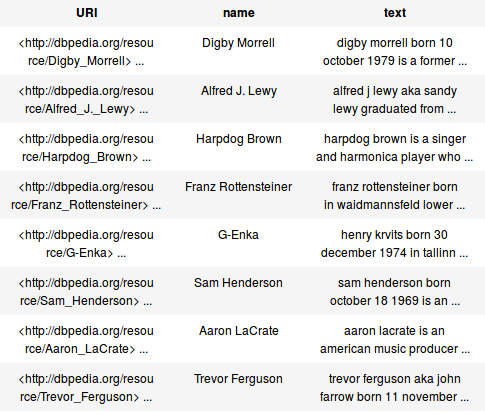
\includegraphics[width=0.9\textwidth, angle=0]{raw_data.jpg}
  \end{center}
\end{figure}

\chapter{Analyses of the data}
\label{chpt:tasks}

\section{Data preparation}

As a preparation we add a new column to the dataset containing the calculated word-count vectors.\\

The GaphLab Create method 'text\_analytics.count\_words' splits the text on all space and new-line characters and uses each unique word as a key with its count in the text as the value. A short preview of the modified dataset can bee seen in figure \ref{fig:dataset}. The following tasks will mainly be manipulating and using this new column, as it is much easier then analysing the whole raw text.\\

\begin{figure}[H]
  \begin{center}
    \caption{Preview of the dataset with an additional column for word counts.}
    \label{fig:dataset}
    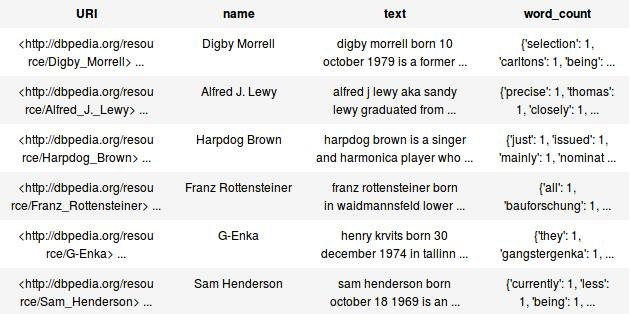
\includegraphics[width=0.9\textwidth, angle=0]{db_wiki_word_counts.jpg}
  \end{center}
\end{figure}

One can already argue now, that the most frequent words will be unimportant words like 'and', 'a' and 'the'. We will see later on how to deal with this and favor more important key words.\\

\section{A first model}

The word counts allow us to define a distance between two articles. As a first model we use the unmodified word counts and the Euclidean distance to be able to tell which articles are the closest to one given article.\\

\noindent
The Euclidian distance is defined as
\begin{center}
\begin{equation}
\label{eq:eu}
D(x, y) = \sqrt{ \sum^d_i (x_i - y_i)^2 }
\end{equation}
\end{center}  
where $d$ is the number of unique words in both articles and $x_i$, $y_i$ are their corresponding counts. If a word only exists in one of the articles it has a value of $0$ in the other. This distance is obviously zero if, and only if, all word counts are the same for two not empty articles.\\

This easy model, using the unmodified word counts, already gets a lot of things right. The ten closest articles to the Barack Obama text are all about politicians. On the other hand some of them have rather tenuous connections with Obama. For example the top 10 include two politicians from the 70ties, another one from Canada, one from Mexico and a British diplomat.\\

These inaccuracies can partially be explained when looking at the top used words from the compared articles. One of the top 10 closest persons to Barack Obama is Francisco Barrio. Table \ref{tab:compare_top_words} compares the top words of the Barack Obama and Francisco Barrio articles sorted by the most common words in Obamas' article. It gets clear by looking at these word counts, that the most frequent words have no value for the comparison of the article and we should find a way to weight the words according to their value for the comparison.\\

To make the problem even more clear, we looked at how many articles are using all of the top 5 words of table \ref{tab:compare_top_words}. Using issubset, we checked whether a set containing the top 5 words is a subset of the word vectors' keyset of each article. It turns out that 56066 out of the 59071 articles include all of the top 5 words. We have to place greater emphasis on rarer and more important words.\\

\begin{table}[H]
  \caption{Comparison of the top words of the Barack Obama and Francisco Barrio articles}
  \label{tab:compare_top_words}
  \begin{center}
    \begin{tabular}{| c | c | c |}
      \hline
      \textbf{Word} & \textbf{Obama} & \textbf{Barrio}\\
      \hline
      \hline
      the & 40 & 36 \\ \hline
      in & 30 & 17 \\ \hline
      and & 21 & 18 \\ \hline
      of & 18 & 24 \\ \hline
      to & 14 & 9 \\ \hline
      his & 11 & 5 \\ \hline
      he & 7 & 10 \\ \hline
      a & 7 & 6 \\ \hline
      as & 6 & 5 \\ \hline
      was & 5 & 4 \\ \hline
    \end{tabular}	
  \end{center}
\end{table}

\section{TF-IDF - A new metric}

Term frequency–inverse document frequency (TF-IDF) calculates a value for each word by comparing the frequency of the word in a specific document with the total number of documents and the number of documents that include the word.\\

\begin{center}
\begin{equation}
\label{eq:td-idf}
TF-IDF(w,d)=tf(w,d) \cdot \log \left( \frac{N}{f(w)} \right),
\end{equation}
\end{center}
\noindent
where $tf(w,d)$ is the number of times word $w$ appeared in document $d$, $f(w)$ is the number of documents word $w$ appeared in and $N$ is the number of documents (from the GraphLab Create documentation). Using this algorithm will lower the impact of words like 'the', because they appear in almost every article and will make rarer and more significant words stand out. Words like 'democrats' will influence the search for closest neighbors more then they did before.\\

For later use we calculate TF-IDF values for every article and save them in a new column. With these new dictionaries we create a new model that should be better in finding neighbors of Obama then the raw model was before. The top 10 neighbors with the new model include only one person that was not an american politician during Obamas time!\\

\section{Cosine distances}

Looking at the equation for the euclidean distance (Eq. \ref{eq:eu}) between two documents, we see that shorter articles will be prefered over longer ones. Longer articles will simply have more word counts in total, which leades to a higher difference in word counts and thus to a larger eucliean distance.\\

Figure \ref{length_1} visualises this preferation of shorter articles. Because of their smaller word counts in general, shorter articles are prefered over longer ones, which might be closer to the topic. The one marked neighbor with a high word count is the Barack Obama article itself.\\

To treat short and long articles equally, we will use Cosine distances for our next model.

\begin{center}
\begin{equation}
D(x,y)=1 - \frac{\sum_i^d x_i \cdot y_i }{\sqrt{\sum_i^d x_i^2 } \cdot \sqrt{\sum_i^d y_i^2 }}, 
\end{equation}
\end{center}
\noindent
As you can see the Cosine distance is divided by the length of the word count vector. This way the length of the article will not influence the measurement, as can be seen in figure \ref{fig:length_2}. With the new distances, our closest neighbors are scattered all over the axis representing the article legth.\\  

\begin{figure}[H]
  \begin{center}
    \caption{Comparison of all document lengths with the lengths of the top 100 nearest neighbors of Obamas article using Euclidean distances.}
    \label{fig:length_1}
    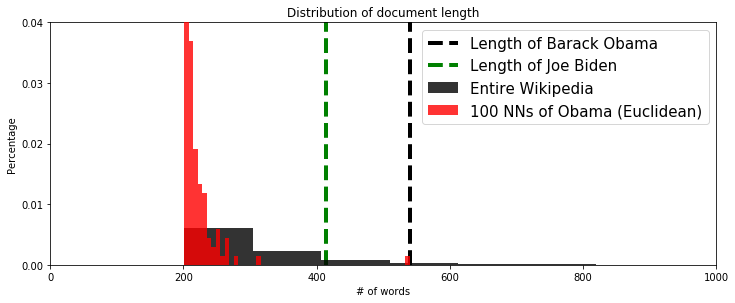
\includegraphics[width=0.9\textwidth, angle=0]{output_70_0.png}
  \end{center}
\end{figure}


\begin{figure}[H]
  \begin{center}
    \caption{Comparison of all document lengths with the lengths of the top 100 nearest neighbors of Obamas article using Cosine distances.}
    \label{fig:length_2}
    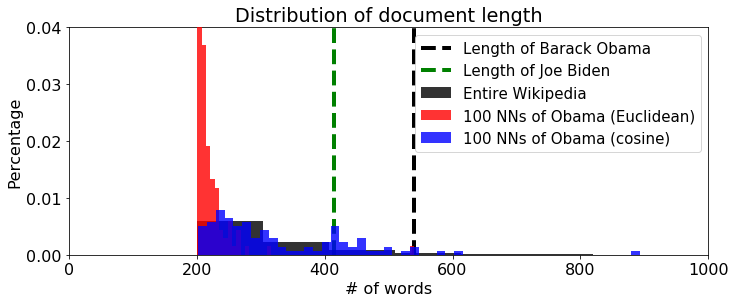
\includegraphics[width=0.9\textwidth, angle=0]{output_78_1.png}
  \end{center}
\end{figure}

\section{Problem with cosine distances}

Now that the lengths of the compared documents do not count anymore, there are some considerations one should make. If the total word count does not matter at all we could get very good matches between completely different types of documents. For example a Tweet containing a lot of key words could be a very good match to the wikipedia article of Barack Obama. In most cases you wouln't want to recommend such a tweet to someone reading a long article.\\

This is why in practise one should set limits on the word counts of the documents that are compared. If we would say for examle, that we only consider documents with a length between one quater of and four times of the length of the querried article, we would be comparing all documents of the dataset, but would have excluded the example of a Tweet.\\

Of course one could also consider hardcoded maximum and minimum word counts for all compared documents, but the probosed flexible range would be able to compare a Tweet to other Tweets and a long article to other longer articles at the same time.\\

\end{document}